\chapter{Introduction to normal mixture models}


%% it 1
\section{Definitions}

A good and thorough introductory book is the work of McLachlan and Peel 2000 and the reader is encouraged to study that to learn in depth about normal mixtures. We will here give a short overwiev of normal mixtures to fix notation and nomenclature.

Let $ \mu \in \mathbb{R}^p , \quad \Sigma \in \mathbb{R}^{p \times p} $ and $ \phi(- ; \mu, \Sigma) $ be the normal distribution with mean $ \mu $ and covariance matrix $ \Sigma $.

Normal mixture model are designed for situations where we assume that a given dataset originates from more than one population of explaining variables.

$ \pmb{Y}_1, \dots , \pmb{Y}_n $

\begin{definition}
    Suppose we have a random sample $ \pmb{Y}_1, \dots , \pmb{Y}_n $ with probability density function $ \pmb{Y}_j \sim f(y_j) $ on $\mathbb{R}^p$ We assume that the density $ f(y_j) $ of $ \pmb{Y}_j $ can be written in the form 

    \[ f(y_j) = \sum_{i=1}^{K} \pi_i \phi_i (y_i; \mu, \Sigma) \]

    The $ \pi_i $ are called the component densities of the mixture.
\end{definition}

explain in scetch EM algo

EM has desirable qualities like proven convergence, (give reference to dempster 1977 paper)

explain idea to use parameter optimizer instead, EM has pathological insufficiencies, like 'getting stuck' for many iterations. We hope we need less iterations, and as concequence less time. 'special' idea: using cholesky decomp.


\section{choice of notation}

describe difference in notation between ceuleux \& govaert and our covariance matrix decomposition.

The classification of models in this paper relies heavily on the work of Celeux and Grovaert, however, out of necessity for clarity, we break with their notation. So as to not confuse the reader we describe here in depth the differences in notation between Celeux and Govaert and ours.

explanation for the volume, shape and orientation descriptors

The basis of classification in CnG is the decomposition of a symmetric matrix into an orthogonal and a diagonal component. A symmetric positive definite matrix $ \Sigma $ can be decomposed as follows 
    \[ \Sigma = \lambda \pmb{D} \pmb{A} \pmb{D}^{\top} \]
with $ \pmb{D} $ an orthogonal matrix and $ \pmb{A} $ a diagonal matrix and $ \lambda = \sqrt[\uproot{3}p]{det(\Sigma)} $ the $ p-th $ root of the determinant of $ \Sigma $.

This decomposition has an appealing geometric interpretation, with $ \pmb{D} $ as the \textit{orientation} of the distribution, $ \pmb{A} $ the \textit{shape}, and $ \lambda $ the \textit{volume}. The problem of notation comes from standard conventions in linear algebra, where the letters $A$ and $D$ are usually occupied by arbytrary and diagonal matrices respectively. Furthermore, we intend to apply a variant of the Cholesky decomposition to $ \Sigma $, the $ \pmb{L}\pmb{D}\pmb{L}^{\top} $ decomposition. This obviously raises some conflicts in notation.

Therefore we, from here on, when reffering to the decomposition as described by cng, will use the following modification of notation:

\begin{align*} 
    \pmb{D} \longmapsto \pmb{Q} \\
    \pmb{A} \longmapsto \pmb{\Lambda} \\
    \lambda \longmapsto \alpha  \\
    \Sigma = \lambda \pmb{D} \pmb{A} \pmb{D}^{\top} =
        \alpha \pmb{Q} \pmb{\Lambda} \pmb{Q}^{\top}
\end{align*}

These were chosen according to general conventions of linear algebra. $ \pmb{Q} $ is usually chosen for orthonormal matrices; $ \pmb{\Lambda} $ is often a choice for eigen vectors and $ \alpha $ was somewhat arbitrarily chosen.


make clear that the models can not be translated one to one to ldlt model

make nice table(maybe sideways to account for parameter list)


\begin{table}[!htb]
    \centering
\rotatebox{90}
{
    \begin{tabular}{| c | c c c c c c | c c c |}
        \hline
        Model & $\pmb{\Sigma}_k$ C\&G & volume & shape & orientation & parameters & count & $ \pmb{LDL}^\top $ & parameters & count \\
        \hline

        EII    & $ \alpha \pmb{I} $ & equal & equal & - & $ \alpha $ & 1 & same as C\&G & & \\
        VII    & $ \alpha_k \pmb{I} $         & variable & equal & - & $ \alpha_k $ & $ K $ & & & \\
        EEI    & $ \alpha \pmb{\Lambda} $     & equal & equal & coordinate axes & $ \alpha, \lambda_i $ & $ 1+p $ & & & \\
        VEI    & $ \alpha_k \pmb{\Lambda} $ & variable & equal & coordinate axes & $ \alpha_k, \lambda_{i}$ & $ K+p $ & & & \\
        EVI    & $ \alpha \pmb{\Lambda}_k $ &equal & variable & coordinate axes & $ \alpha, \lambda_{i,k} $ & $ 1+pK $ & & & \\
        VVI    & $ \alpha_k \pmb{\Lambda}_k $ & variable & variable & coordinate axes & $ \alpha_k, \lambda_{i,k} $ & $ K+pK $ & & & \\
        \hline
        EEE    & $ \alpha \pmb{Q \Lambda Q}^\top $ &equal & equal & equal & $ \alpha, \lambda_{i}, q_{i,j} $ & $ 1+p+p^2 $ & $ \alpha \pmb{LDL}^{\top} $ & & \\
        \hline
        EVE    & $ \alpha \pmb{Q \Lambda}_k \pmb{Q}^\top $ &equal & variable & equal & $ \alpha, \lambda_{i,k}, q_{i,j} $ & $ 1+pK+p^2 $ & doesn't exist & & \\
        \hline
        VEE    & $ \alpha_k \pmb{Q \Lambda Q}^\top $ & variable & equal & equal & $ \alpha_k, \lambda_{i}, q_{i,j} $ & $ K+p+p^2 $ & $ \alpha_k \pmb{LDL}^\top $ & & \\
        \hline
        VVE    & $ \alpha_k \pmb{Q \Lambda}_k \pmb{Q}^\top $ &variable & variable & equal & $ \alpha_k, \lambda_{i,k}, q_{i,j} $ & $ K+pK+p^2 $ & & & \\
        EEV    & $ \alpha \pmb{Q}_k \pmb{\Lambda} \pmb{Q}_k^\top $ &equal & equal & variable & $ \alpha, \lambda_{i}, q_{i,j,k} $ & $ 1+p+Kp^2 $ &    & & \\
        VEV    & $ \alpha_k \pmb{Q}_k \pmb{\Lambda} \pmb{Q}_k^\top $ &variable & equal & variable & $ \alpha_k, \lambda_{i}, q_{i,j,k} $ & $ K+p+Kp^2 $ & & & \\
        \hline
        EVV    & $ \alpha \pmb{Q}_k \pmb{\Lambda}_k \pmb{Q}_k^\top $ & equal & variable & variable & $ \alpha, \lambda_{i}, q_{i,j,k} $ & $ 1+pK+Kp^2 $ & $ \alpha \pmb{L}_k \pmb{D}_k \pmb{L}_k^\top $ & $ \lambda, d_{i,k}, l_{i,j,k}\ j>i $ & $ 1+pK+K\frac{p(p-1)}{2} $ \\
        VVV    & $ \alpha_k \pmb{Q}_k \pmb{\Lambda}_k \pmb{Q}_k^\top $ & variable & variable & variable & $ \alpha_k, \lambda_{i}, q_{i,j,k} $ & $ K+pK+Kp^2 $ & $ \alpha_k \pmb{L}_k \pmb{D}_k \pmb{L}_k^\top $ & $ \lambda_k, d_{i,k}, l_{i,j,k}\ j>i $ & $ K+pK+K\frac{p(p-1)}{2} $ \\
        \hline
    \end{tabular}

    \label{table:1}

}

\caption{Table of Parameters}

\end{table}


\clearpage

\section{problems of EM}


the EM algo has stalling problems especially close to a local optimum

show an example using nor1mix



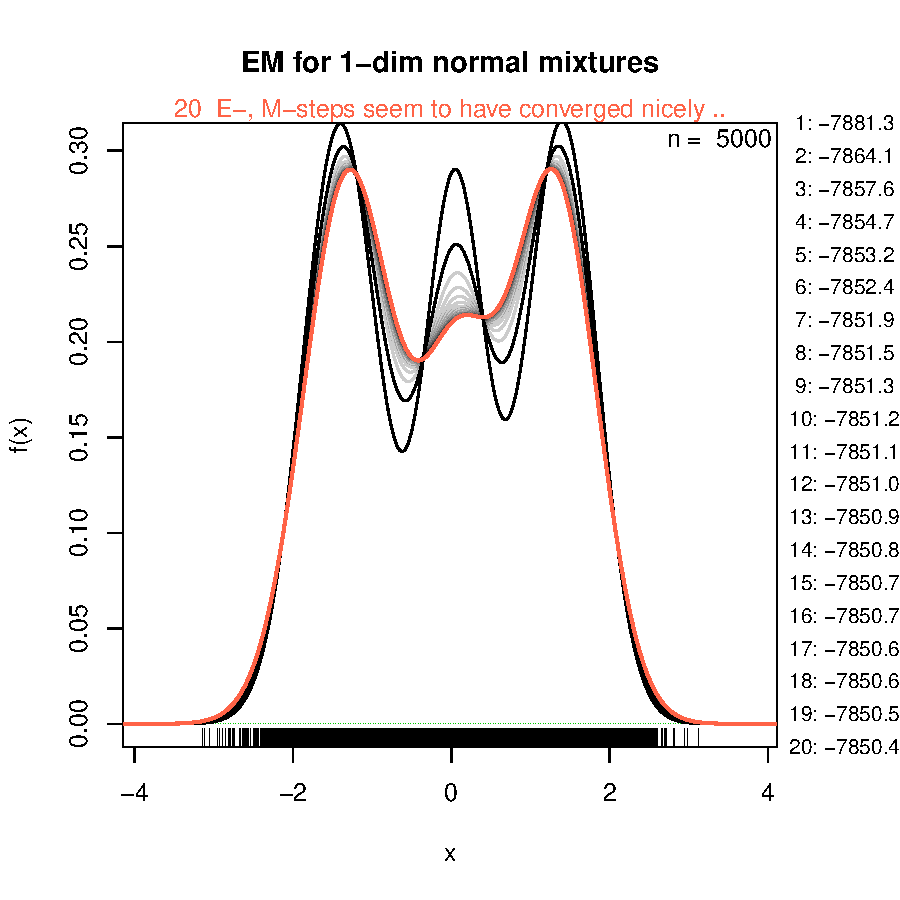
\includegraphics{chapter1-002}



then an illustration of MW examples of pathological cases


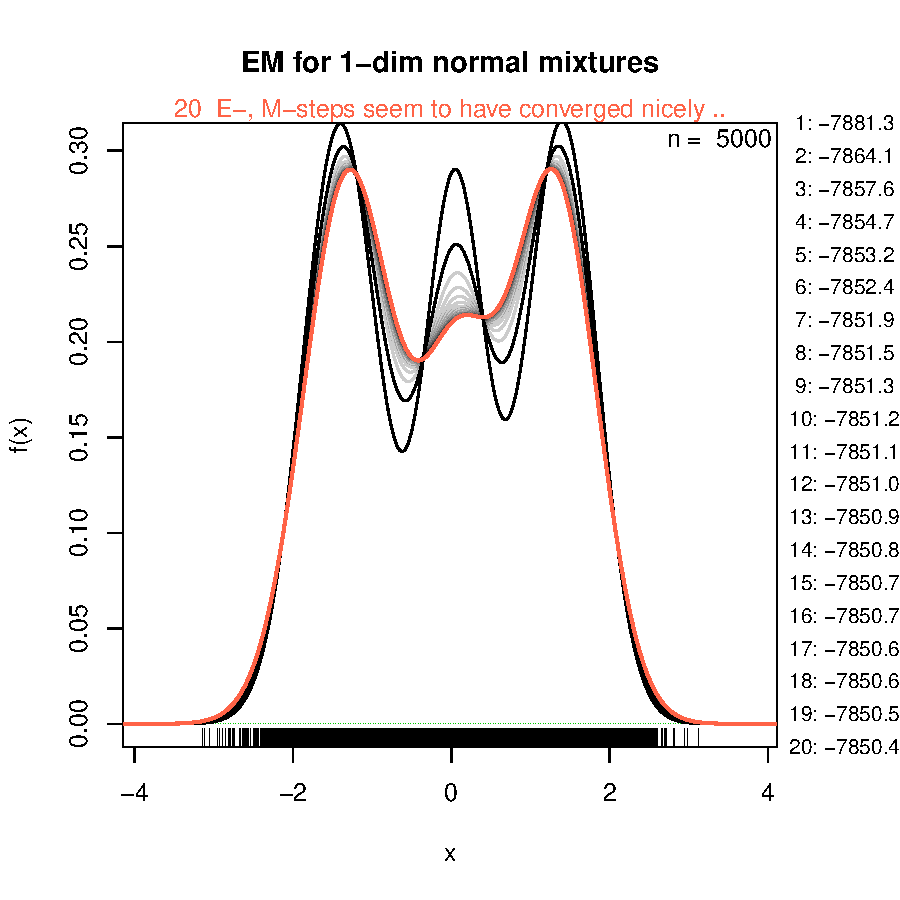
\includegraphics{chapter1-nor1mixEx}


yay, got figure to print. solution was use of fig=TRUE, instead of various mutations like figure=true.

here we see how change in loglik seems to stagnate. However, this does not stay that way, if we let EM run a bit further.


\begin{figure}
\begin{center}
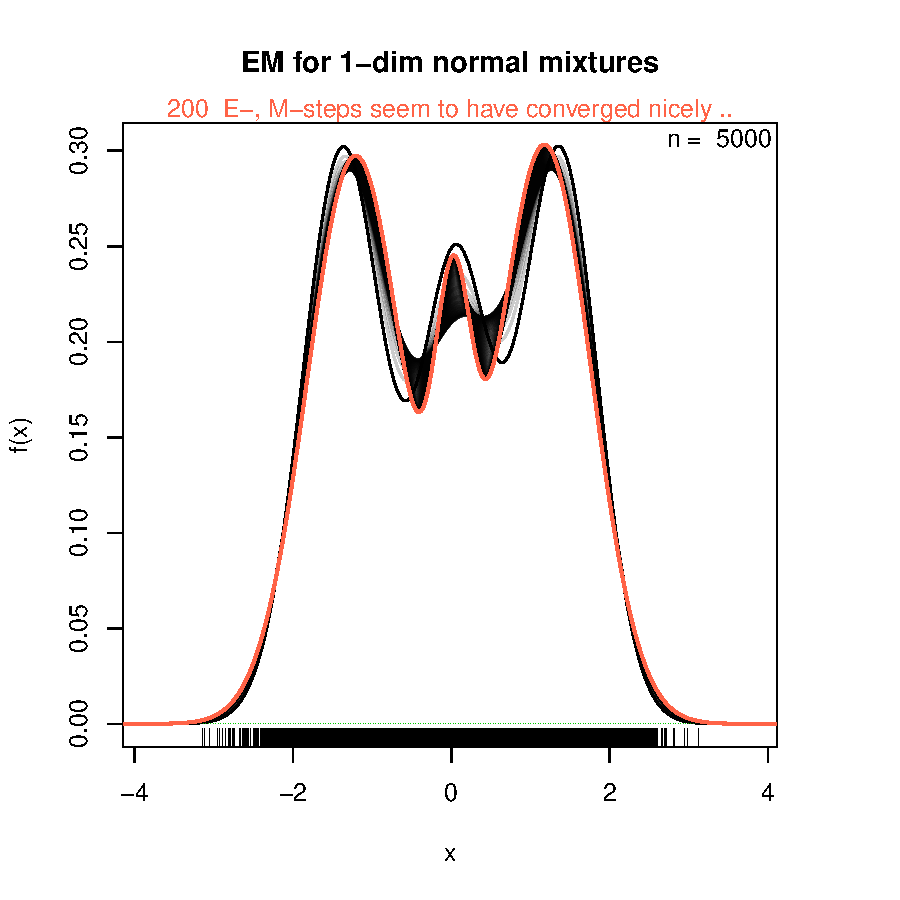
\includegraphics{chapter1-005}
\end{center}
\caption{200 EM steps}
\label{adfafdafds}
\end{figure}

to conclude example show part of mixest that shows it takes 1200 iterations to converge

In fact, it seems that the previous solution is a saddle point in the likelihood function, where EM has chronic problems continuing improvements.

should include animations?? like mix\_est\_1d.R line 249+24 lines

maybe show Marr Wand's examples of 'difficult' mixtures

give conclusion recapping the just demonstrated, and lead in for next chapter






\chapter{The {\tt norMmix} Package}

explain, that this package was written purposefully for this paper.

The norMmix package is constructed around the {\tt norMmix} object, that codifies a {\tt nor}mal {\tt M}ultivariate {\tt mix}ture model,  and the {\tt llnorMmix()} function.

quickly list contents of norMmix object

relies on {\tt optim()} generic optimizer. maximizes llnormix by varying model parameters.

since mclust is one of the more popular packages implementing the EM algo, we employ a lot of functions from mclust, to keep things around EM as similar as possible.

also relies on {\tt mixtools} package for random generating function {\tt rnorMmix} using {\tt rmvnorm}.

\section{concept of package} (this Section maybe one chapter earlier)

about Cholesky decomp as ldlt. has advantages: fast, parametrically parsimonious, can easily compute loglikelihood

maybe reread section in McLachlan about accelerating EM algo

not possible to sensibly compare normal mixtures except maybe a strange sorting algorithm using mahalanobis distance or Kullback-Leibler distance or similar(Hellinger), but not numerically sensible to integrate over potentially high-dimensional spaces.

So caomparison of algos done through throwing difficult mixtures and non-mixtures at it and hoping that norMmix finds better solutions than EM. So the criteria for "better fit" are 1. better log-likelihood 2. correct model, where EM fails.

\section{finer details of {\tt norMmix} package}




\chapter{Comparing Algotithms}

display abilities of norMmix on its own. can find correct models

maybe apply to MW[0-9] objects?

not sure

as in Raftery2002, Benaglia2009, Roeder 1997, maybe compare to MISE of various forms. They all did and see it as adequate method for comparing accuracy of algorithm.

also wanted is accuracy of model selection. generate from model and then compare fitted to original. either by acc-model==fit-model and acc-k==fit-k or acc-ll - fit-ll.


\chapter{Conclusions}

testing citations
\cite{McL00} \cite{Ben09} \cite{Roe97}
